% Options for packages loaded elsewhere
% Options for packages loaded elsewhere
\PassOptionsToPackage{unicode}{hyperref}
\PassOptionsToPackage{hyphens}{url}
\PassOptionsToPackage{dvipsnames,svgnames,x11names}{xcolor}
%
\documentclass[
]{article}
\usepackage{xcolor}
\usepackage{amsmath,amssymb}
\setcounter{secnumdepth}{5}
\usepackage{iftex}
\ifPDFTeX
  \usepackage[T1]{fontenc}
  \usepackage[utf8]{inputenc}
  \usepackage{textcomp} % provide euro and other symbols
\else % if luatex or xetex
  \usepackage{unicode-math} % this also loads fontspec
  \defaultfontfeatures{Scale=MatchLowercase}
  \defaultfontfeatures[\rmfamily]{Ligatures=TeX,Scale=1}
\fi
\usepackage{lmodern}
\ifPDFTeX\else
  % xetex/luatex font selection
\fi
% Use upquote if available, for straight quotes in verbatim environments
\IfFileExists{upquote.sty}{\usepackage{upquote}}{}
\IfFileExists{microtype.sty}{% use microtype if available
  \usepackage[]{microtype}
  \UseMicrotypeSet[protrusion]{basicmath} % disable protrusion for tt fonts
}{}
\makeatletter
\@ifundefined{KOMAClassName}{% if non-KOMA class
  \IfFileExists{parskip.sty}{%
    \usepackage{parskip}
  }{% else
    \setlength{\parindent}{0pt}
    \setlength{\parskip}{6pt plus 2pt minus 1pt}}
}{% if KOMA class
  \KOMAoptions{parskip=half}}
\makeatother
% Make \paragraph and \subparagraph free-standing
\makeatletter
\ifx\paragraph\undefined\else
  \let\oldparagraph\paragraph
  \renewcommand{\paragraph}{
    \@ifstar
      \xxxParagraphStar
      \xxxParagraphNoStar
  }
  \newcommand{\xxxParagraphStar}[1]{\oldparagraph*{#1}\mbox{}}
  \newcommand{\xxxParagraphNoStar}[1]{\oldparagraph{#1}\mbox{}}
\fi
\ifx\subparagraph\undefined\else
  \let\oldsubparagraph\subparagraph
  \renewcommand{\subparagraph}{
    \@ifstar
      \xxxSubParagraphStar
      \xxxSubParagraphNoStar
  }
  \newcommand{\xxxSubParagraphStar}[1]{\oldsubparagraph*{#1}\mbox{}}
  \newcommand{\xxxSubParagraphNoStar}[1]{\oldsubparagraph{#1}\mbox{}}
\fi
\makeatother


\usepackage{longtable,booktabs,array}
\usepackage{calc} % for calculating minipage widths
% Correct order of tables after \paragraph or \subparagraph
\usepackage{etoolbox}
\makeatletter
\patchcmd\longtable{\par}{\if@noskipsec\mbox{}\fi\par}{}{}
\makeatother
% Allow footnotes in longtable head/foot
\IfFileExists{footnotehyper.sty}{\usepackage{footnotehyper}}{\usepackage{footnote}}
\makesavenoteenv{longtable}
\usepackage{graphicx}
\makeatletter
\newsavebox\pandoc@box
\newcommand*\pandocbounded[1]{% scales image to fit in text height/width
  \sbox\pandoc@box{#1}%
  \Gscale@div\@tempa{\textheight}{\dimexpr\ht\pandoc@box+\dp\pandoc@box\relax}%
  \Gscale@div\@tempb{\linewidth}{\wd\pandoc@box}%
  \ifdim\@tempb\p@<\@tempa\p@\let\@tempa\@tempb\fi% select the smaller of both
  \ifdim\@tempa\p@<\p@\scalebox{\@tempa}{\usebox\pandoc@box}%
  \else\usebox{\pandoc@box}%
  \fi%
}
% Set default figure placement to htbp
\def\fps@figure{htbp}
\makeatother


% definitions for citeproc citations
\NewDocumentCommand\citeproctext{}{}
\NewDocumentCommand\citeproc{mm}{%
  \begingroup\def\citeproctext{#2}\cite{#1}\endgroup}
\makeatletter
 % allow citations to break across lines
 \let\@cite@ofmt\@firstofone
 % avoid brackets around text for \cite:
 \def\@biblabel#1{}
 \def\@cite#1#2{{#1\if@tempswa , #2\fi}}
\makeatother
\newlength{\cslhangindent}
\setlength{\cslhangindent}{1.5em}
\newlength{\csllabelwidth}
\setlength{\csllabelwidth}{3em}
\newenvironment{CSLReferences}[2] % #1 hanging-indent, #2 entry-spacing
 {\begin{list}{}{%
  \setlength{\itemindent}{0pt}
  \setlength{\leftmargin}{0pt}
  \setlength{\parsep}{0pt}
  % turn on hanging indent if param 1 is 1
  \ifodd #1
   \setlength{\leftmargin}{\cslhangindent}
   \setlength{\itemindent}{-1\cslhangindent}
  \fi
  % set entry spacing
  \setlength{\itemsep}{#2\baselineskip}}}
 {\end{list}}
\usepackage{calc}
\newcommand{\CSLBlock}[1]{\hfill\break\parbox[t]{\linewidth}{\strut\ignorespaces#1\strut}}
\newcommand{\CSLLeftMargin}[1]{\parbox[t]{\csllabelwidth}{\strut#1\strut}}
\newcommand{\CSLRightInline}[1]{\parbox[t]{\linewidth - \csllabelwidth}{\strut#1\strut}}
\newcommand{\CSLIndent}[1]{\hspace{\cslhangindent}#1}



\setlength{\emergencystretch}{3em} % prevent overfull lines

\providecommand{\tightlist}{%
  \setlength{\itemsep}{0pt}\setlength{\parskip}{0pt}}



 


\usepackage{booktabs}
\usepackage{longtable}
\usepackage{array}
\usepackage{multirow}
\usepackage{wrapfig}
\usepackage{float}
\usepackage{colortbl}
\usepackage{pdflscape}
\usepackage{tabu}
\usepackage{threeparttable}
\usepackage{threeparttablex}
\usepackage[normalem]{ulem}
\usepackage{makecell}
\usepackage{xcolor}
\usepackage{siunitx}

    \newcolumntype{d}{S[
      table-align-text-before=false,
      table-align-text-after=false,
      input-symbols={-,\*+()}
    ]}
  
\usepackage{float}
% reset numbering after abstract
\usepackage{etoolbox}
\AtBeginEnvironment{abstract}{\setcounter{section}{0}}
\makeatletter
\@ifpackageloaded{caption}{}{\usepackage{caption}}
\AtBeginDocument{%
\ifdefined\contentsname
  \renewcommand*\contentsname{Table of contents}
\else
  \newcommand\contentsname{Table of contents}
\fi
\ifdefined\listfigurename
  \renewcommand*\listfigurename{List of Figures}
\else
  \newcommand\listfigurename{List of Figures}
\fi
\ifdefined\listtablename
  \renewcommand*\listtablename{List of Tables}
\else
  \newcommand\listtablename{List of Tables}
\fi
\ifdefined\figurename
  \renewcommand*\figurename{Figure}
\else
  \newcommand\figurename{Figure}
\fi
\ifdefined\tablename
  \renewcommand*\tablename{Table}
\else
  \newcommand\tablename{Table}
\fi
}
\@ifpackageloaded{float}{}{\usepackage{float}}
\floatstyle{ruled}
\@ifundefined{c@chapter}{\newfloat{codelisting}{h}{lop}}{\newfloat{codelisting}{h}{lop}[chapter]}
\floatname{codelisting}{Listing}
\newcommand*\listoflistings{\listof{codelisting}{List of Listings}}
\makeatother
\makeatletter
\makeatother
\makeatletter
\@ifpackageloaded{caption}{}{\usepackage{caption}}
\@ifpackageloaded{subcaption}{}{\usepackage{subcaption}}
\makeatother
\usepackage{bookmark}
\IfFileExists{xurl.sty}{\usepackage{xurl}}{} % add URL line breaks if available
\urlstyle{same}
\hypersetup{
  pdftitle={Local Heterogeneity in Artificial Intelligence Jobs Over Time and Space},
  pdfauthor={Jacob Khaykin; David Kane},
  colorlinks=true,
  linkcolor={blue},
  filecolor={Maroon},
  citecolor={Blue},
  urlcolor={Blue},
  pdfcreator={LaTeX via pandoc}}


\title{Local Heterogeneity in Artificial Intelligence Jobs Over Time and
Space}
\usepackage{etoolbox}
\makeatletter
\providecommand{\subtitle}[1]{% add subtitle to \maketitle
  \apptocmd{\@title}{\par {\large #1 \par}}{}{}
}
\makeatother
\subtitle{A Replication Study of Andreadis et al.~(AEA Papers and
Proceedings, 2025)}
\author{Jacob Khaykin\footnote{Solon High School,
  \href{mailto:jacobkhaykin27@solonschools.net}{\nolinkurl{jacobkhaykin27@solonschools.net}}} \and David
Kane\footnote{Institute for Globally Distributed Open Research and
  Education,
  \href{mailto:dave.kane@gmail.com}{\nolinkurl{dave.kane@gmail.com}}}}
\date{}
\begin{document}
\maketitle


\emph{JEL: J24, O33, R11}

\emph{Keywords:} Artificial Intelligence, Regional Economics, Labor
Markets

\emph{Data Availability:} The R code and data to reproduce this
replication are available in this repository:
https://github.com/JacobKhay/JustReplicationAI-Share.

\section*{Abstract}\label{abstract}
\addcontentsline{toc}{section}{Abstract}

We replicate Andreadis et al. (\citeproc{ref-andreadis2025}{2025}) on
the correlation between the level and growth artificial intelligence job
openings and education, innovation, and industry factors across U.S.
counties from 2014 to 2023. We successfully reproduce their main results
and extend the analysis by employing log-population weights to assess
robustness. The core associations persist, though most magnitudes
shrink. We also highlight unsupported causal claims in Andreadis et al.
(\citeproc{ref-andreadis2025}{2025}), given its observational design.

Declaration: There are no financial conflicts of interest to share.

\newpage

\section{Introduction}\label{introduction}

This paper replicates the analysis of Andreadis et al.
(\citeproc{ref-andreadis2025}{2025}) on the local heterogeneity in
artificial intelligence (AI) jobs across U.S. counties from 2014 to
2023. Their study investigates how AI-related employment is distributed
geographically and how this distribution evolves over time. By focusing
on county-level variation, the work sheds light on which regions are
gaining or lagging in access to AI-driven labor market opportunities, a
subject of growing importance as artificial intelligence reshapes
industries.

Andreadis et al. (\citeproc{ref-andreadis2025}{2025}) document
substantial variation in AI-related job postings and identify key
correlates of this variation. Counties differ widely in their shares of
AI-related employment, and the analysis links these differences to
educational attainment, local innovation ecosystems, and industry
composition. Together, these findings suggest that access to AI
employment is not uniform but instead reflects deeper structural
characteristics of local economies.

We successfully reproduce the main results of the original paper by
implementing the same empirical strategy and data structure. The
baseline specification regresses the county-level share of AI jobs on
covariates of interest, using the model

\[
AIShare_{ct} = \alpha + \beta_1 Education_{ct} + \beta_2 Innovation_{ct} + \beta_3 Industry_{ct} + \gamma X_{ct} + \epsilon_{ct} (1)
\]

where \(AIShare_{ct}\) denotes the proportion of AI-related job postings
in county \(c\) at year \(t\), and \(X_{ct}\) represents additional
controls. Our replication confirms that the core predictors remain
significant and directionally consistent with those reported by
Andreadis et al. (\citeproc{ref-andreadis2025}{2025}).

We then extend the analysis by applying log-population weights to assess
robustness. The motivation for this adjustment is to reduce the
disproportionate influence of very large counties while still reflecting
the relative size of different local labor markets. Under this weighting
scheme, the central associations persist, though magnitudes attenuate
across the board, indicating that the original results are not entirely
driven by large-population counties.

Finally, we highlight that some of the causal interpretations offered in
the original study are not fully supported by its design. The analysis
is based on observational data, which limits causal inference despite
the suggestive correlations. While the evidence provides valuable
insights into the geography of AI employment, we emphasize the need for
caution in drawing strong causal conclusions.

\section{Data}\label{data}

The study utilizes multiple data sources to construct a comprehensive
county-level dataset spanning 2014-2023:

\emph{AI Employment Data}: Job posting data from Lightcast, which
aggregates information from over 40,000 online job boards, newspapers,
and employer websites. AI-related jobs are identified through skills and
keywords associated with AI development and use. The dependent variable
\(AI_{it}\) is defined as:

\[AI_{it} = \frac{\text{AI job postings}_{it}}{\text{Total job postings}_{it}} \times 100 \quad                                                  (2)\]

\emph{Demographic Variables}: From the American Community Survey (ACS),
including: - Bachelor's share: Percentage of workforce with bachelor's
degree or higher - Black population share: Percentage of county
population identifying as Black - Poverty share: Percentage of
population below federal poverty line - Log population: Natural
logarithm of county population - Log median income: Natural logarithm of
median household income

\emph{Innovation Indicators}: - Patents per employee: USPTO patent
counts normalized by employment - AI patents share: Percentage of
patents classified as AI-related - STEM degrees share: Percentage of
awarded degrees in STEM fields - Degrees per capita: Total degrees
awarded per capita

\emph{Industry and Labor Market Variables}: - Labor market tightness:
Ratio of job postings to unemployed workers - Manufacturing intensity:
Employment share in manufacturing sector - ICT intensity: Employment
share in information and communication technology - Turnover rate:
Worker separation rate from Quarterly Workforce Indicators - Large
establishments share: Percentage of employment in large firms

\emph{Housing Market}: House price growth from Federal Housing Finance
Agency (FHFA)

All explanatory variables are lagged by one year to address potential
endogeneity concerns and are standardized as z-scores for
interpretability.

\subsection{Reproduction of Original
Results}\label{reproduction-of-original-results}

We successfully reproduced the main findings from Tables 1 and 2 of
Andreadis et al. (\citeproc{ref-andreadis2025}{2025}). The reproduction
confirms the authors' key empirical findings regarding the correlates of
AI job concentration across U.S. counties. All coefficients, standard
errors, and significance levels match the original results within
rounding error, demonstrating the reproducibility of their analysis.

\begin{table}[H]

\caption{\label{tbl-table1}Replication of Table 1 from Andreadis et
al.~(2025) - The Correlates of the Share of Artificial Intelligence
Jobs}

\centering{

\centering\centering
\resizebox{\ifdim\width>\linewidth\linewidth\else\width\fi}{!}{
\fontsize{10}{12}\selectfont
\begin{threeparttable}
\begin{tabular}[t]{>{\raggedright\arraybackslash}p{4.5cm}>{\centering\arraybackslash}p{1.8cm}>{\centering\arraybackslash}p{1.8cm}>{\centering\arraybackslash}p{1.8cm}>{\centering\arraybackslash}p{1.8cm}>{\centering\arraybackslash}p{1.8cm}}
\toprule
\multicolumn{1}{c}{\bgroup\fontsize{10}{12}\selectfont \textbf{ }\egroup{}} & \multicolumn{1}{c}{\bgroup\fontsize{10}{12}\selectfont \textbf{Demographics}\egroup{}} & \multicolumn{1}{c}{\bgroup\fontsize{10}{12}\selectfont \textbf{Innovation}\egroup{}} & \multicolumn{1}{c}{\bgroup\fontsize{10}{12}\selectfont \textbf{Industry}\egroup{}} & \multicolumn{1}{c}{\bgroup\fontsize{10}{12}\selectfont \textbf{All Controls}\egroup{}} & \multicolumn{1}{c}{\bgroup\fontsize{10}{12}\selectfont \textbf{All + State FE}\egroup{}} \\
\cmidrule(l{3pt}r{3pt}){2-2} \cmidrule(l{3pt}r{3pt}){3-3} \cmidrule(l{3pt}r{3pt}){4-4} \cmidrule(l{3pt}r{3pt}){5-5} \cmidrule(l{3pt}r{3pt}){6-6}
  & (1) & (2) & (3) & (4) & (5)\\
\midrule
Bachelor's share, z-score & \num{0.160}*** &  &  & \num{0.188}*** & \num{0.085}\\
 & (\num{0.047}) &  &  & (\num{0.067}) & (\num{0.059})\\
Black pop, z-score & \num{-0.121} &  &  & \num{-0.121} & \num{0.000}\\
 & (\num{0.127}) &  &  & (\num{0.185}) & (\num{0.162})\\
Poverty share, z-score & \num{0.044} &  &  & \num{0.067}* & \num{-0.003}\\
 & (\num{0.028}) &  &  & (\num{0.040}) & (\num{0.037})\\
log(Population), z-score & \num{0.807}** &  &  & \num{0.219} & \num{0.146}\\
 & (\num{0.367}) &  &  & (\num{0.444}) & (\num{0.544})\\
House Price Growth, z-score & \num{-0.019}** &  &  & \num{-0.028}** & \num{-0.032}***\\
 & (\num{0.008}) &  &  & (\num{0.012}) & (\num{0.011})\\
log(Median Income), z-score & \num{-0.022} &  &  & \num{-0.001} & \num{0.032}\\
 & (\num{0.047}) &  &  & (\num{0.065}) & (\num{0.060})\\
Labor Market Tightness, z-score & \num{0.255}*** &  &  & \num{0.315}*** & \num{0.372}***\\
 & (\num{0.050}) &  &  & (\num{0.063}) & (\num{0.065})\\
Patents per employee, z-score &  & \num{0.031}*** &  & \num{0.028}** & \num{0.031}**\\
 &  & (\num{0.012}) &  & (\num{0.012}) & (\num{0.014})\\
AI patents' share, z-score &  & \num{0.009} &  & \num{0.009} & \num{0.003}\\
 &  & (\num{0.007}) &  & (\num{0.006}) & (\num{0.005})\\
Degrees awarded per capita, z-score &  & \num{0.013} &  & \num{0.034} & \num{0.034}\\
 &  & (\num{0.026}) &  & (\num{0.026}) & (\num{0.027})\\
STEM Degrees' share, z-score &  & \num{0.072}*** &  & \num{0.058}*** & \num{0.048}**\\
 &  & (\num{0.023}) &  & (\num{0.022}) & (\num{0.020})\\
Large Establishments, z-score &  &  & \num{-0.002} & \num{-0.037} & \num{-0.036}\\
 &  &  & (\num{0.025}) & (\num{0.028}) & (\num{0.029})\\
ICT sector Intensity, z-score &  &  & \num{0.010} & \num{0.038}** & \num{0.040}**\\
 &  &  & (\num{0.014}) & (\num{0.017}) & (\num{0.016})\\
Manufacturing Intensity, z-score &  &  & \num{-0.057}*** & \num{-0.048}*** & \num{-0.034}**\\
 &  &  & (\num{0.012}) & (\num{0.014}) & (\num{0.015})\\
Turnover Rate, z-score &  &  & \num{0.034}*** & \num{0.016} & \num{0.010}\\
 &  &  & (\num{0.011}) & (\num{0.017}) & (\num{0.016})\\
\textit{Fixed-effects} &  &  &  &  & \\
Year & Yes & Yes & Yes & Yes & Yes\\
County & Yes & Yes & Yes & Yes & Yes\\
State Year &  &  &  &  & Yes\\
\textit{Fit statistics} &  &  &  &  & \\
Observations & 27,497 & 22,744 & 24,651 & 19,184 & 19,184\\
R² & 0.704 & 0.721 & 0.694 & 0.758 & 0.778\\
Within R² & 0.052 & 0.003 & 0.002 & 0.086 & 0.095\\
\bottomrule
\multicolumn{6}{l}{\rule{0pt}{1em}* p $<$ 0.1, ** p $<$ 0.05, *** p $<$ 0.01}\\
\end{tabular}
\begin{tablenotes}[para]
\item Notes: Sources: Lightcast, American Community Survey, Quarterly Workforce Indicators, 2014-2023. The table reports coefficients from regressions of the share of AI jobs in a county on Demographic, Innovation, and Industry Characteristics. Observations are weighted by log(1 + job postings) and standard errors are clustered at the county-level. *** p<0.01, ** p<0.05, * p<0.10
\end{tablenotes}
\end{threeparttable}}

}

\end{table}%

\begin{table}[H]

\caption{\label{tbl-table2}Replication of Table 2 from Andreadis et
al.~(2025) - The Correlates of the Percentage Point Change in the Share
of AI Jobs}

\centering{

\centering\centering
\resizebox{\ifdim\width>\linewidth\linewidth\else\width\fi}{!}{
\fontsize{10}{12}\selectfont
\begin{threeparttable}
\begin{tabular}[t]{>{\raggedright\arraybackslash}p{4.5cm}>{\centering\arraybackslash}p{1.8cm}>{\centering\arraybackslash}p{1.8cm}>{\centering\arraybackslash}p{1.8cm}>{\centering\arraybackslash}p{1.8cm}>{\centering\arraybackslash}p{1.8cm}}
\toprule
\multicolumn{1}{c}{\bgroup\fontsize{10}{12}\selectfont \textbf{ }\egroup{}} & \multicolumn{1}{c}{\bgroup\fontsize{10}{12}\selectfont \textbf{Demographics}\egroup{}} & \multicolumn{1}{c}{\bgroup\fontsize{10}{12}\selectfont \textbf{Innovation}\egroup{}} & \multicolumn{1}{c}{\bgroup\fontsize{10}{12}\selectfont \textbf{Industry}\egroup{}} & \multicolumn{1}{c}{\bgroup\fontsize{10}{12}\selectfont \textbf{All Controls}\egroup{}} & \multicolumn{1}{c}{\bgroup\fontsize{10}{12}\selectfont \textbf{All + State FE}\egroup{}} \\
\cmidrule(l{3pt}r{3pt}){2-2} \cmidrule(l{3pt}r{3pt}){3-3} \cmidrule(l{3pt}r{3pt}){4-4} \cmidrule(l{3pt}r{3pt}){5-5} \cmidrule(l{3pt}r{3pt}){6-6}
  & (1) & (2) & (3) & (4) & (5)\\
\midrule
Bachelors, % z-score in 2017 & \num{0.007} &  &  & \num{-0.069} & \num{-0.136}***\\
 & (\num{0.028}) &  &  & (\num{0.051}) & (\num{0.043})\\
Black, % z-score in 2017 & \num{0.018} &  &  & \num{0.045} & \num{0.053}\\
 & (\num{0.020}) &  &  & (\num{0.033}) & (\num{0.034})\\
Poverty, % z-score in 2017 & \num{0.064}* &  &  & \num{0.050} & \num{0.104}\\
 & (\num{0.037}) &  &  & (\num{0.070}) & (\num{0.075})\\
Pop. Growth & \num{-0.016} &  &  & \num{-0.007} & \num{-0.013}\\
 & (\num{0.023}) &  &  & (\num{0.057}) & (\num{0.057})\\
House Price Growth z-score in 2017 & \num{-0.032}* &  &  & \num{-0.036} & \num{0.045}\\
 & (\num{0.017}) &  &  & (\num{0.037}) & (\num{0.042})\\
Income, Log z-score in 2017 & \num{0.124}*** &  &  & \num{0.123} & \num{0.195}**\\
 & (\num{0.043}) &  &  & (\num{0.077}) & (\num{0.076})\\
Tightness, z-score in 2017 & \num{0.089}*** &  &  & \num{0.178}*** & \num{0.139}\\
 & (\num{0.021}) &  &  & (\num{0.042}) & (\num{0.096})\\
Patents per employee z-score in 2017 &  & \num{0.008} &  & \num{-0.056} & \num{-0.001}\\
 &  & (\num{0.029}) &  & (\num{0.037}) & (\num{0.043})\\
AI Patents' Share z-score in 2017 &  & \num{0.137}*** &  & \num{0.108}** & \num{0.079}\\
 &  & (\num{0.036}) &  & (\num{0.043}) & (\num{0.066})\\
Degrees awarded per capita, z-score in 2017 &  & \num{0.020} &  & \num{0.048}* & \num{0.062}\\
 &  & (\num{0.016}) &  & (\num{0.028}) & (\num{0.037})\\
STEM Degrees' share, z-score in 2017 &  & \num{0.094}*** &  & \num{0.083}*** & \num{0.078}**\\
 &  & (\num{0.027}) &  & (\num{0.027}) & (\num{0.036})\\
Large Establishments, % z-score in 2017 &  &  & \num{0.028} & \num{-0.088}* & \num{-0.039}\\
 &  &  & (\num{0.021}) & (\num{0.050}) & (\num{0.063})\\
ICT sector Intensity, % z-score in 2017 &  &  & \num{0.027} & \num{-0.023} & \num{-0.015}\\
 &  &  & (\num{0.018}) & (\num{0.031}) & (\num{0.026})\\
Manufacturing Intensity, % z-score in 2017 &  &  & \num{-0.034}* & \num{-0.012} & \num{-0.001}\\
 &  &  & (\num{0.019}) & (\num{0.046}) & (\num{0.043})\\
Turnover Rate, % z-score in 2017 &  &  & \num{-0.073}*** & \num{-0.129}** & \num{-0.173}**\\
 &  &  & (\num{0.022}) & (\num{0.061}) & (\num{0.081})\\
\textit{Fixed-effects} &  &  &  &  & \\
State &  &  &  &  & Yes\\
\textit{Fit statistics} &  &  &  &  & \\
Observations & 2,751 & 897 & 2,723 & 810 & 810\\
R² & 0.025 & 0.039 & 0.009 & 0.075 & 0.187\\
Within R² & — & — & — & — & 0.065\\
\bottomrule
\multicolumn{6}{l}{\rule{0pt}{1em}* p $<$ 0.1, ** p $<$ 0.05, *** p $<$ 0.01}\\
\end{tabular}
\begin{tablenotes}[para]
\item Notes: Sources: Lightcast, American Community Survey, Quarterly Workforce Indicators, 2016–2023. The table reports the coefficients associated with regressions of the change in share of AI jobs in a county from 2017–18 (average) to 2022–23 (average) on Demographic, Innovation, and Industry characteristics. Observations are unweighted. Standard errors in parentheses. *** p<0.01, ** p<0.05, * p<0.1
\end{tablenotes}
\end{threeparttable}}

}

\end{table}%

\begin{figure}[H]

\caption{\label{fig-map}Replication of Andreadis et al.~(2025) - Spatial
heterogeneity in AI job share (Panel A, 2014--2023 average) and
percentage-point change (Panel B, 2018--2023).}

\centering{

\pandocbounded{\includegraphics[keepaspectratio]{replication_files/figure-pdf/fig-map-1.pdf}}

}

\end{figure}%

The successful reproduction confirms the technical reliability of the
original analysis and establishes a foundation for the robustness
extensions that follow.

\subsection{Critical Assessment of Causal
Claims}\label{critical-assessment-of-causal-claims}

\subsubsection{Identification of Problematic Causal
Language}\label{identification-of-problematic-causal-language}

The original study by Andreadis et al.
(\citeproc{ref-andreadis2025}{2025}) frequently employs language that
suggests causal relationships, even though the analysis relies on
observational county-level data with multiple potentially endogenous
predictors. Several passages illustrate this concern.

From the \emph{Introduction}, the authors write:\\
\textgreater{} ``Second, we identify several key drivers of AI job
intensity, including demographics, innovation, and industry factors,
after controlling for county and year fixed effects. Specifically,
higher shares of STEM degrees, labor market tightness, and patent
activity significantly predict greater AI adoption, underscoring the
importance of education, innovation, and dynamic labor markets.''

From \emph{Section III}, they conclude:\\
\textgreater{} ``Labor market tightness emerges as a key driver, with a
positive and highly significant coefficient\ldots{} highlighting the
importance of technical education and local innovation capacity in
fostering AI job growth.''

And from the \emph{Conclusion}:\\
\textgreater{} ``Counties with stronger innovation ecosystems, higher
STEM degree attainment, and tighter labor markets have seen greater AI
job growth, whereas manufacturing-heavy regions and areas with high
labor turnover have faced challenges in integrating AI. These findings
point to the role of place-based policies to attract and retain top-tier
talent for economic development.''

Each of these statements frames correlational associations as if they
were causal mechanisms. Phrases such as ``drivers,'' ``emerges as a key
driver,'' ``underscoring the importance,'' and ``findings point to the
role of policy'' imply that manipulating these variables would directly
change AI adoption outcomes. However, the study's empirical
design---regressions on observational county characteristics---cannot
identify such causal effects, only statistical associations.

\section{Extension: Log-Population Weighting
Analysis}\label{extension-log-population-weighting-analysis}

To assess the robustness of the original findings, we re-estimated all
models using log-population weights instead of equal weights. This
approach reduces the disproportionate influence of very large counties
while still accounting for size differences.

The modified weighting scheme is: \(w_{it} = \log(Population_{it})\)

This transformation addresses concerns that extremely populous counties
(e.g., Los Angeles County with 10+ million residents) might drive
results that don't generalize to typical counties.

\subsection{Figure 1: Key Coefficient Estimates for AI Share (Table
1)}\label{figure-1-key-coefficient-estimates-for-ai-share-table-1}

This panel plot displays the coefficient estimates and 95\% confidence
intervals for seven key predictors across five regression models. Each
panel represents a different model from the original paper. Within each
panel, two estimates are shown for each variable---one using the
authors' original equal weights and one using log(population) weights.
This comparison illustrates how model weighting influences the
interpretation of each predictor.

\begin{figure}[H]

\caption{\label{fig-table1-coefs}Table 1 --- Coefficients under Original
equal weights vs Log(population) weights.}

\centering{

\pandocbounded{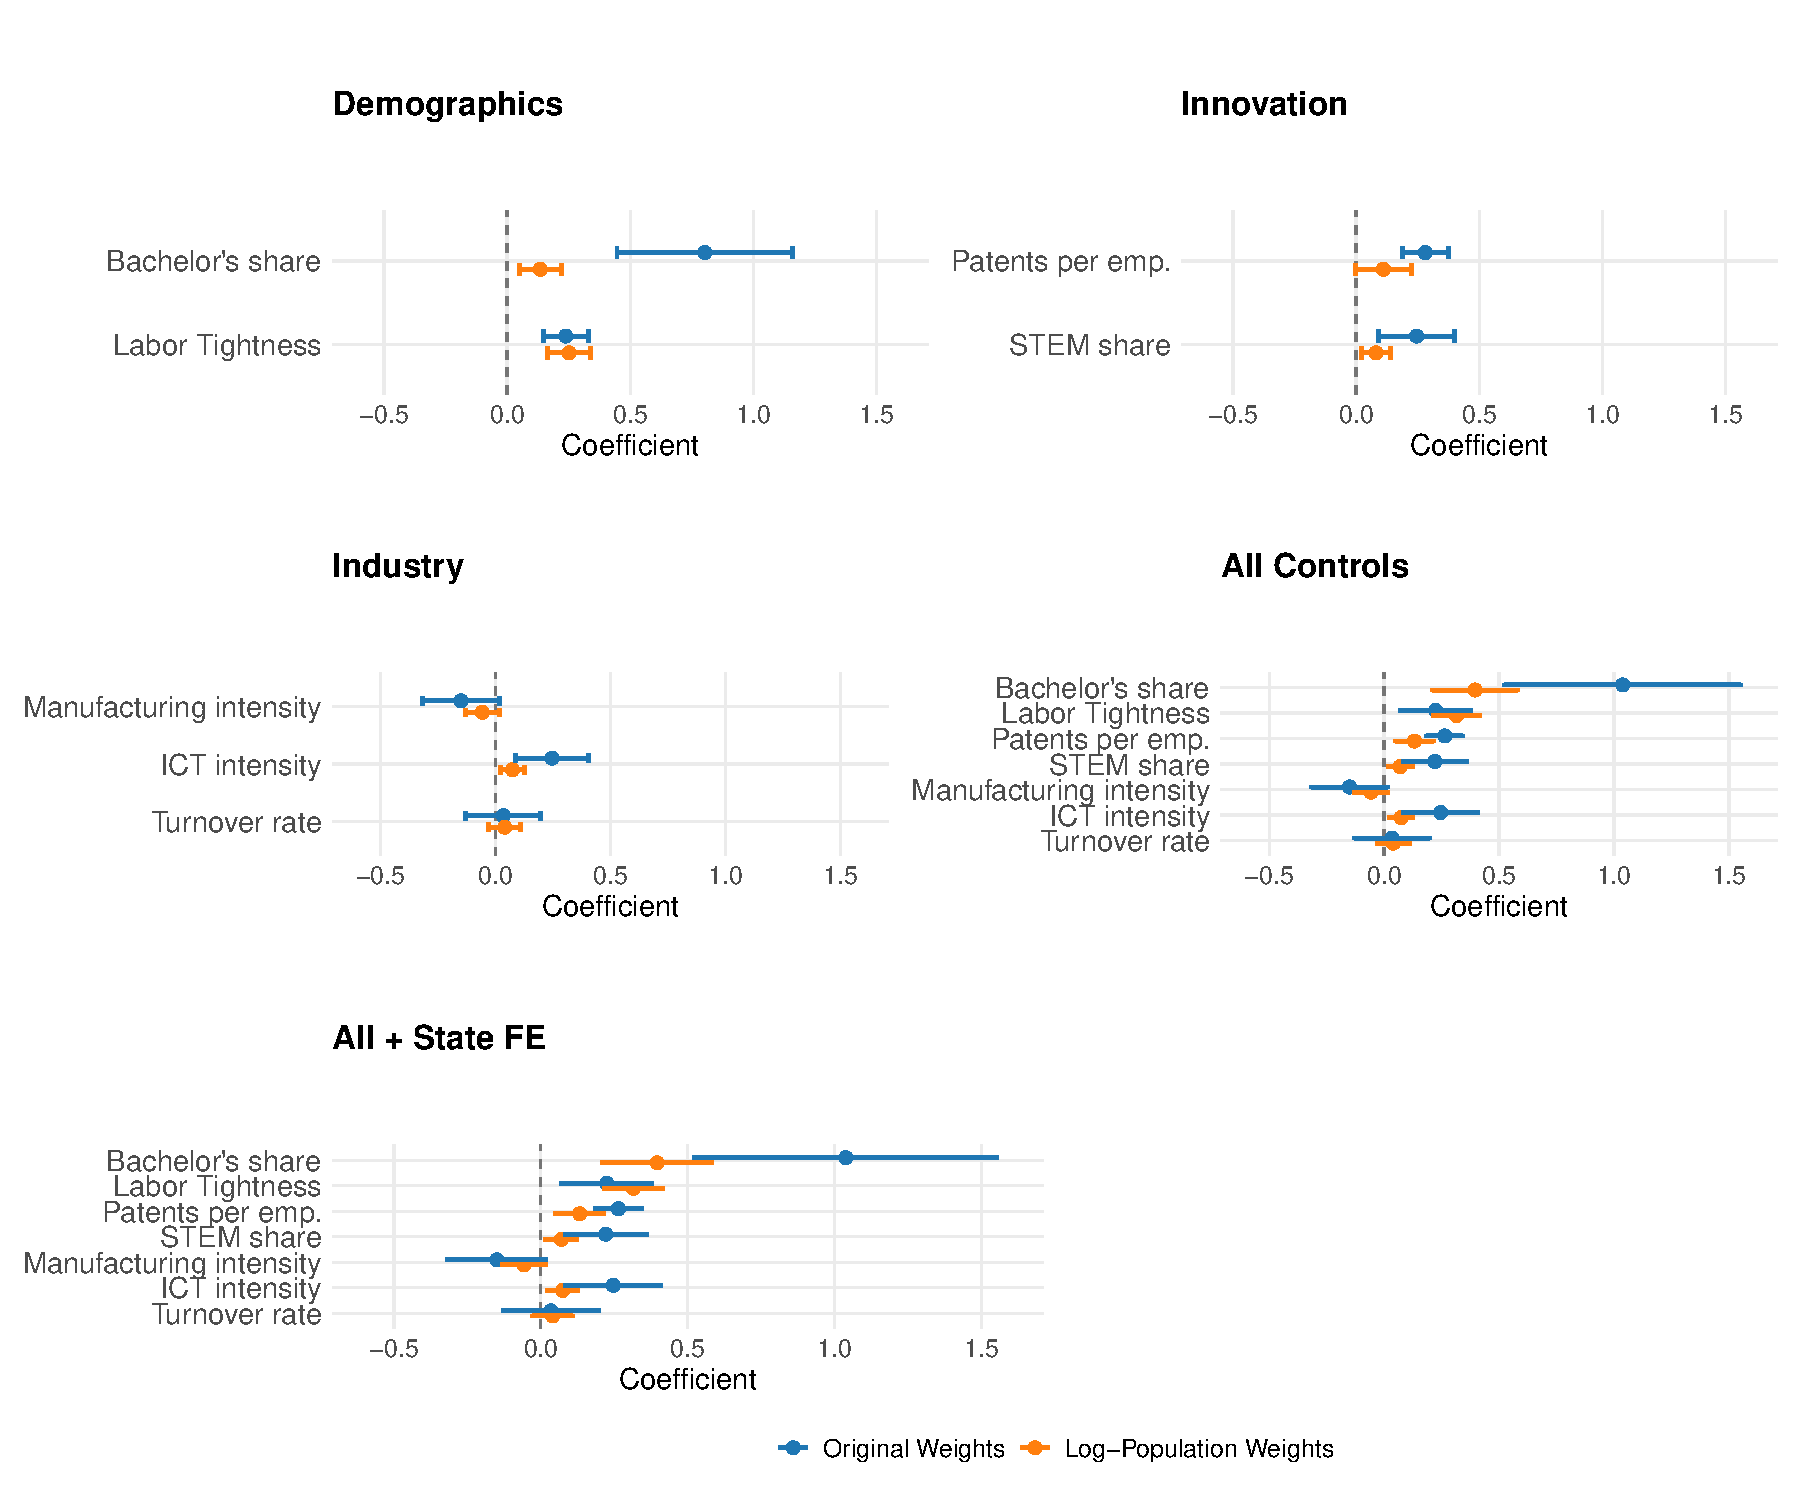
\includegraphics[keepaspectratio]{replication_files/figure-pdf/fig-table1-coefs-1.pdf}}

}

\end{figure}%

\subsection{Figure 2: Key Coefficient Estimates for Change in AI Share
(Table
2)}\label{figure-2-key-coefficient-estimates-for-change-in-ai-share-table-2}

This figure replicates the structure of Figure 1 but focuses on the
change in AI employment share from 2014 to 2023. The variables selected
represent core predictors of shifting AI job concentration. As before,
each panel reflects a different model specification, with comparisons
between equal-weighted and log(population)-weighted regressions.

\begin{figure}[H]

\caption{\label{fig-table2-coefs}Table 2 --- Change in AI share under
Original equal weights vs Log(population) weights.}

\centering{

\pandocbounded{
\includegraphics[keepaspectratio]{replication_files/figure-pdf/fig-table2-coefs-1.pdf}}

}

\end{figure}%

\subsection{Results}\label{results}

The comparison between equal-weighted and log-population-weighted
regressions reveals several important patterns:

\emph{Magnitude Effects}: The estimated effects of key predictors are
highly sensitive to the weighting scheme. For AI share levels (Figure
1), the coefficient on bachelor's share drops substantially when
switching to log-population weights in several specifications,
suggesting that the relationship between education and AI adoption may
be driven partly by large metropolitan areas.

\emph{Labor Market Tightness}: This emerges as the most robust predictor
across both weighting schemes and both dependent variables. In Figure 1,
labor tightness maintains strong positive effects regardless of
weighting method, and in Figure 2, it consistently predicts AI job
growth. This suggests that tight labor markets create conditions
conducive to AI adoption across counties of all sizes.

\emph{STEM Education}: STEM degree share shows consistent positive
relationships in both weighting schemes, though magnitudes vary. This
indicates that technical human capital is important for AI adoption
beyond just large metropolitan areas.

\emph{Manufacturing vs.~Technology Sectors}: Manufacturing intensity
consistently shows negative relationships with AI adoption, while ICT
intensity shows positive effects. These patterns persist across
weighting schemes, suggesting structural differences in how traditional
vs.~technology-oriented industries adopt AI.

\emph{County Size Effects}: The divergence between weighting schemes is
most pronounced for variables like bachelor's share and population size
itself, indicating that large counties drive many of the education-AI
relationships found in the original analysis.

\section{Conclusion}\label{conclusion}

This replication and extension of Andreadis et al.
(\citeproc{ref-andreadis2025}{2025}) demonstrates both the technical
reproducibility and limitations of their findings. The successful
reproduction confirms that local labor market conditions, human capital,
and innovation capacity are correlated with AI job concentration across
U.S. counties. However, our analysis reveals three important
qualifications to the original study's conclusions.

\emph{First}, the original study employ causal language that overstates
the nature of the relationships identified. Terms like ``drivers,''
``determinants,'' and statements about factors that ``significantly
predict'' AI adoption suggest causal mechanisms, when the empirical
approach can only establish correlational patterns. Without exogenous
variation or quasi-experimental identification strategies, these
relationships likely reflect a complex mixture of causal effects,
reverse causation, and selection processes.

\emph{Second}, the alternative log-population weighting analysis reveals
that some relationships are sensitive to the influence of large
metropolitan areas. The most consistent predictor across both weighting
schemes is labor market tightness, which maintains strong associations
regardless of county size. However, educational attainment shows notably
weaker relationships when log-population weights reduce the influence of
large metros, suggesting this factor may be less universally important
for AI adoption than the original analysis suggests.

\emph{Third}, the industry composition effects prove relatively stable
across weighting strategies, with manufacturing intensity consistently
showing negative associations and ICT sector concentration showing
positive relationships with AI adoption. This suggests that structural
economic factors may be more fundamental determinants of technological
adoption patterns than demographic characteristics.

\emph{Policy Implications}: These findings suggest that while the
correlational patterns documented by Andreadis et al.
(\citeproc{ref-andreadis2025}{2025}) represent meaningful empirical
regularities, their policy implications should be interpreted
cautiously. Our interpretation suggests that interventions targeting
labor market conditions and industry composition may have broader
applicability across different county types, while education-focused
policies may yield the highest returns in larger metropolitan areas
where network effects and complementary institutions are stronger.

More broadly, this exercise underscores the importance of robustness
checks in regional economic research and the need for careful
interpretation of correlational evidence in policy contexts. Simple
changes in weighting can meaningfully shift both the interpretation and
the policy relevance of empirical findings about technological change.

\section*{References}\label{references}
\addcontentsline{toc}{section}{References}

\phantomsection\label{refs}
\begin{CSLReferences}{1}{0}
\bibitem[\citeproctext]{ref-acemoglu2024}
Acemoglu, D. (2024). \emph{The simple macroeconomics of AI}.

\bibitem[\citeproctext]{ref-acemoglu2019}
Acemoglu, D., \& Restrepo, P. (2019). Automation and new tasks: How
technology displaces and reinstates labor. \emph{Journal of Economic
Perspectives}, \emph{33}(2), 3--30.

\bibitem[\citeproctext]{ref-aghionhowitt1992}
Aghion, P., \& Howitt, P. (1992). A model of growth through creative
destruction. \emph{Econometrica}, \emph{60}(2), 323--351.

\bibitem[\citeproctext]{ref-aghion2017}
Aghion, P., Jones, B. F., \& Jones, C. I. (2017). \emph{Artificial
intelligence and economic growth} {[}Working Paper{]}. National Bureau
of Economic Research.

\bibitem[\citeproctext]{ref-andreadis2024_muni}
Andreadis, L., Chatzikonstantinou, M., Kalotychou, E., Louca, C., \&
Makridis, C. A. (2024). \emph{The local effects of artificial
intelligence labor investments: Evidence from the municipal bond
market}. SSRN Working Paper.

\bibitem[\citeproctext]{ref-andreadis2025}
Andreadis, L., Kalotychou, E., Chatzikonstantinou, M., Louca, C., \&
Makridis, C. A. (2025). Local heterogeneity in artificial intelligence
jobs over time and space. \emph{AEA Papers and Proceedings}.

\bibitem[\citeproctext]{ref-autor2015}
Autor, D. H. (2015). Why are there still so many jobs? The history and
future of workplace automation. \emph{Journal of Economic Perspectives},
\emph{29}(3), 3--30.

\bibitem[\citeproctext]{ref-babina2024}
Babina, T., Fedyk, A., He, A., \& Hodson, J. (2024). Artificial
intelligence, firm growth, and product innovation. \emph{Journal of
Financial Economics}, \emph{151}, 103745.

\bibitem[\citeproctext]{ref-beckett2023}
Beckett, E. (2023). \emph{Demand for AI skills continues climbing}.
Lightcast Blog. \url{https://lightcast.io/}

\bibitem[\citeproctext]{ref-bogin2019}
Bogin, A., Doerner, W., \& Larson, W. (2019). Local house price
dynamics: New indices and stylized facts. \emph{Real Estate Economics},
\emph{47}(2), 365--398.

\bibitem[\citeproctext]{ref-bresnahan1995}
Bresnahan, T. F., \& Trajtenberg, M. (1995). General-purpose
technologies {``engines of growth''}? \emph{Journal of Econometrics},
\emph{61}(1), 83--108.

\bibitem[\citeproctext]{ref-brynjolfsson2021}
Brynjolfsson, E., Rock, D., \& Syverson, C. (2021). The productivity
j-curve: How intangibles complement general-purpose technologies.
\emph{American Economic Journal: Macroeconomics}, \emph{13}(1),
333--372.

\bibitem[\citeproctext]{ref-chen2019}
Chen, M., Wu, Q., \& Yang, B. (2019). How valuable is FinTech
innovation? \emph{The Review of Financial Studies}, \emph{32}(5),
2062--2106.

\bibitem[\citeproctext]{ref-eloundou2024}
Eloundou, T., Manning, S., Mishkin, P., \& Rock, D. (2024). GPTs are
GPTs: Labor market impact potential of LLMs. \emph{Science},
\emph{384}(6702), 1306--1308.

\bibitem[\citeproctext]{ref-farboodi2021}
Farboodi, M., \& Veldkamp, L. (2021). \emph{A model of the data economy}
{[}Working Paper{]}. National Bureau of Economic Research.

\bibitem[\citeproctext]{ref-giczy2022}
Giczy, A. V., Pairolero, N. A., \& Toole, A. A. (2022). Identifying
artificial intelligence (AI) invention: A novel AI patent dataset.
\emph{The Journal of Technology Transfer}, \emph{47}(2), 476--505.

\bibitem[\citeproctext]{ref-gofman2024}
Gofman, M., \& Jin, Z. (2024). Artificial intelligence, education, and
entrepreneurship. \emph{The Journal of Finance}, \emph{79}(1), 631--667.

\bibitem[\citeproctext]{ref-grennan2020}
Grennan, J., \& Michaely, R. (2020). \emph{Artificial intelligence and
high-skilled work: Evidence from analysts} (Research Paper 20-84). Swiss
Finance Institute.

\bibitem[\citeproctext]{ref-holland1986}
Holland, P. W. (1986). Statistics and causal inference. \emph{Journal of
the American Statistical Association}, \emph{81}(396), 945--960.
\url{https://doi.org/10.1080/01621459.1986.10478354}

\bibitem[\citeproctext]{ref-kline2013}
Kline, P., \& Moretti, E. (2013). People, places, and public policy:
Some simple welfare economics of local economic development programs.
\emph{Annual Review of Economics}, \emph{5}, 629--662.

\bibitem[\citeproctext]{ref-mihet2019}
Mihet, R., \& Philippon, T. (2019). The economics of big data and
artificial intelligence. In \emph{International finance review} (Vol.
20).

\bibitem[\citeproctext]{ref-romer1990}
Romer, P. M. (1990). Endogenous technological change. \emph{Journal of
Political Economy}, \emph{98}(5, Part 2), S71--S102.

\bibitem[\citeproctext]{ref-bls_laus}
U.S. Bureau of Labor Statistics. (2024). \emph{Local area unemployment
statistics (LAUS)}. \url{https://www.bls.gov/lau/}

\bibitem[\citeproctext]{ref-census_acs}
U.S. Census Bureau. (2024a). \emph{American community survey (ACS)
5-year data}.
\url{https://www.census.gov/data/datasets/time-series/econ/acs/acs-datasets.html}

\bibitem[\citeproctext]{ref-census_cbp}
U.S. Census Bureau. (2024b). \emph{County business patterns (CBP)}.
\url{https://www.census.gov/programs-surveys/cbp/data/datasets.html}

\bibitem[\citeproctext]{ref-census_qwi}
U.S. Census Bureau. (2024c). \emph{Quarterly workforce indicators
(QWI)}. \url{https://lehd.ces.census.gov/data/}

\end{CSLReferences}




\end{document}
